This project contains 4 big block components:
\begin{itemize}
    \item Controller 
    \item Google Cloud Speech API
    \item OctoPrint
    \item 3D Printer
\end{itemize}

Function of each component:

\begin{itemize}
    \item Controller: Takes speech and .STL file as input.
    \item Google Cloud Speech API: receives speech from user, then converts speech to text. 
In other words, Google Cloud Speech API provides audio transcription.
    \item OctoPrint: interface to adjust settings on the printer and to print object.
    \item 3D Printer: print 3D object from user's commands.
\end{itemize}

Note:

\begin{itemize}
    \item If Google Cloud Speech API does not work out, Google Home API will be used instead.
    \item New components could be added to the system later if needed.
\end{itemize}

\begin{figure}[h!]
	\centering
   	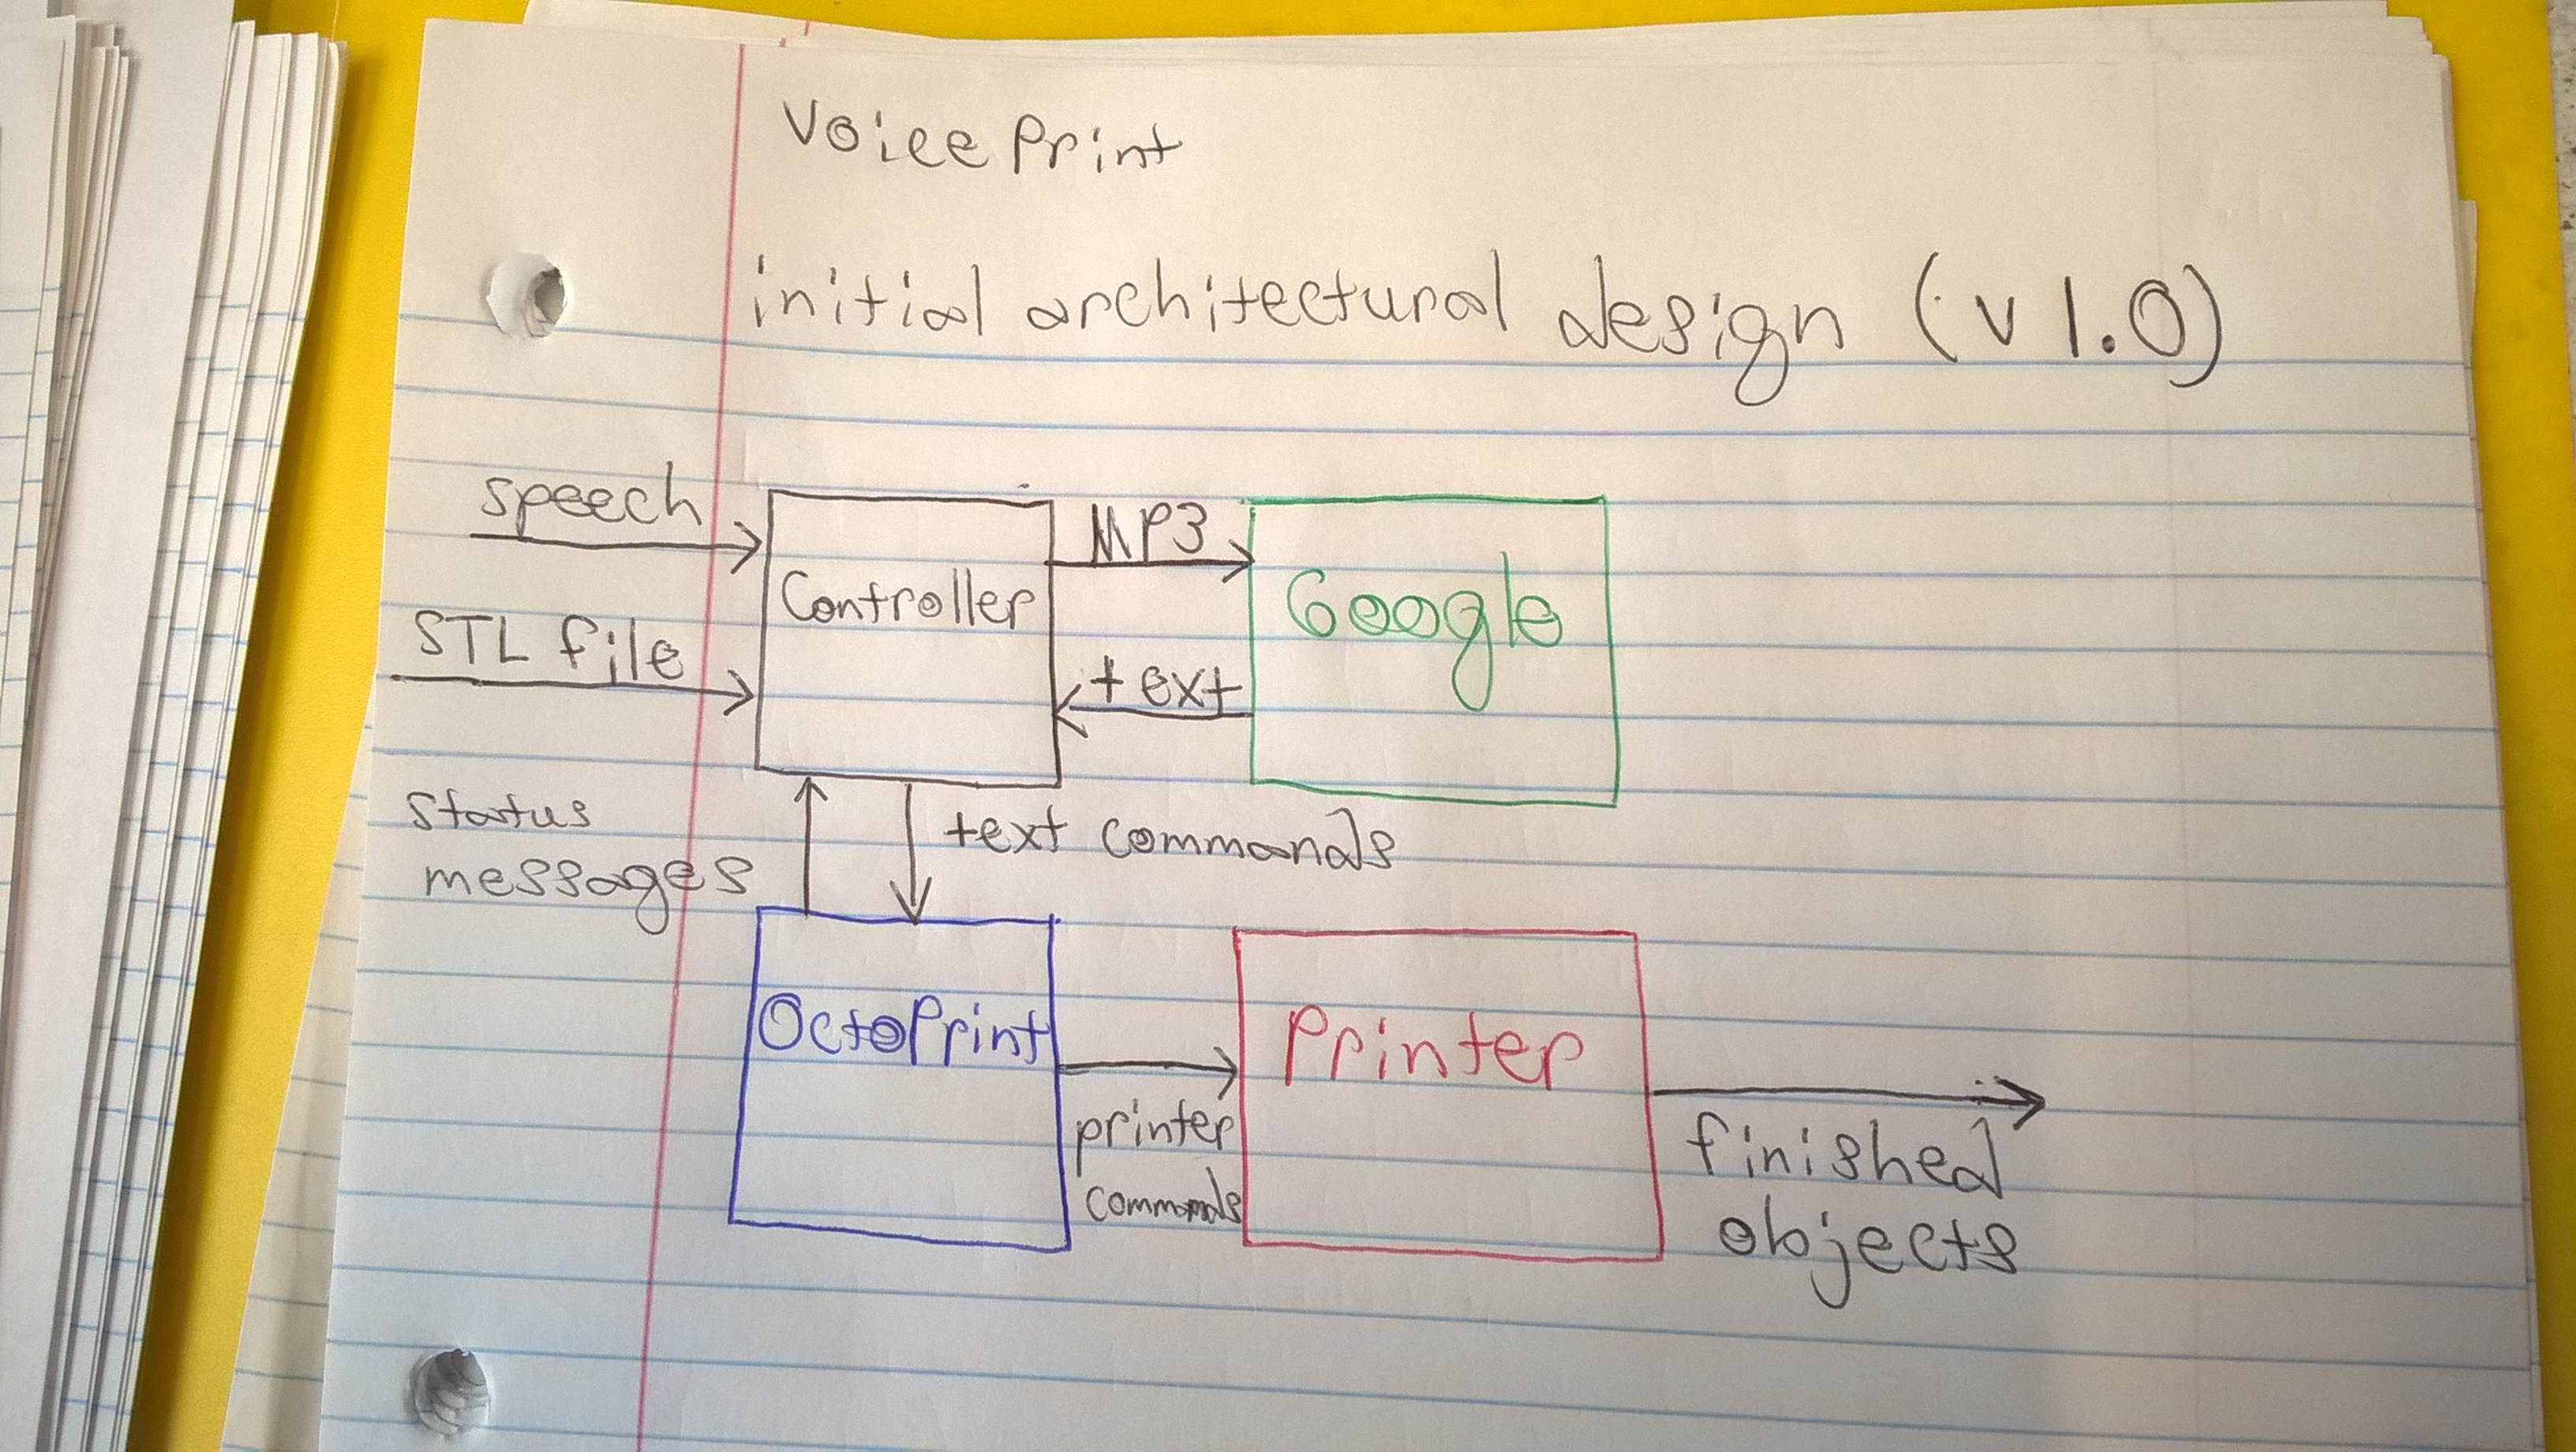
\includegraphics[width=0.7\textwidth]{images/Diagram.jpg}
   	    \caption{Diagram of major components of VoicePrint}
\end{figure}


